\chapter{Phase 3 - Logistical Optimization}
\setcounter{section}{0}
\renewcommand{\thesection}{\arabic{section}}
\label{chap:logistics}

\section*{Introduction}
This chapter marks the transition from "What is in the image?" (Detection) to "What is the object doing?" (Behavior Analysis). While Chapter 3 established the detection foundation for industrial hazards, this chapter focuses on Logistical Intelligence. Specifically, it details the mathematical and architectural mechanisms required to calculate real-time speed and heading angles of industrial vehicles. This transition from static bounding boxes to dynamic behavioral metrics forms the core intelligence of the EYE-D video analytics solution.

\section{Specific State of the Art}
This section presents the foundational theory required for behavioral analysis, focusing on coordinate transformation and temporal smoothing.

\subsection{Homography and Geometric Projection}
\label{subsec:homography}
To calculate real-world velocity from a 2D camera feed, the system must correct for perspective distortion. Pixel-based measurements are inherently flawed because objects farther from the camera appear smaller and move fewer pixels per unit of real-world distance. 

This is addressed using a Homography matrix ($\mathbf{H}$), which mathematically maps coordinates from the 2D image plane to a top-down, real-world 3D coordinate system (projected onto the 2D ground plane). Given a point $(x, y)$ in the image, its corresponding real-world coordinate $(x', y')$ is computed via the transformation:
\begin{equation}
\begin{bmatrix} x' \\ y' \\ 1 \end{bmatrix} = \mathbf{H} \begin{bmatrix} x \\ y \\ 1 \end{bmatrix} = \begin{bmatrix} h_{11} & h_{12} & h_{13} \\ h_{21} & h_{22} & h_{23} \\ h_{31} & h_{32} & h_{33} \end{bmatrix} \begin{bmatrix} x \\ y \\ 1 \end{bmatrix}
\end{equation}
where the final world coordinates $(x', y')$ are directly obtained. The full $3 \times 3$ homography matrix is typically estimated from at least 4 point correspondences using the Direct Linear Transform (DLT) algorithm. By tracking the centroid of an object across consecutive frames and applying this transformation, the system calculates displacement in meters, enabling accurate velocity calculations.

\subsection{Comparison with Existing Calibration Solutions}
To justify the use of homography, it is necessary to critique existing calibration methods commonly employed in industry:

\begin{itemize}
  \item \textbf{Ultralytics YOLO Speed Estimation:} The standard Ultralytics framework provides a built-in speed module that relies on a simplified \texttt{meter\_per\_pixel} parameter for linear pixel-to-meter conversion. This lacks perspective correction entirely, resulting in severe inaccuracies when vehicles move diagonally or further away from the camera lens.
  \item \textbf{Manual Calibration (OpenCV):} Traditional OpenCV-based approaches often utilize simple Euclidean distance formulas between detected object centroids. These require manual specification of scale factors without automatic perspective correction, making them brittle and strictly limited to estimating speed without capturing orientation.
  \item \textbf{Our Homography Implementation:} By computing a proper $3 \times 3$ homography matrix calibrated from four point correspondences, the system provides both speed and heading estimation in true world coordinates, immune to the perspective distortion that breaks simpler linear scaling methods.
\end{itemize}

\subsection{Smoothing \& Tracking}
Raw detections inherently contain jitter (positional noise). If uncorrected, this noise leads to erratic speed spikes and unstable heading angles. To handle detection noise, two primary mechanisms are utilized:

\begin{itemize}
    \item \textbf{Kalman Filters \& ByteTrack:} Object tracking algorithms like ByteTrack rely on Kalman Filters to predict an object's future position based on its current velocity and trajectory. The Kalman Filter continuously updates its internal state, smoothing the bounding box coordinates even when the object is partially occluded.
    \item \textbf{Exponential Moving Average (EMA):} For the final speed and angle outputs, an EMA filter is applied to heavily dampen frame-to-frame jitter. The EMA filter equation is $S_t = \alpha \cdot X_t + (1 - \alpha) \cdot S_{t-1}$, where $S_t$ is the smoothed value, $X_t$ is the raw input, and $\alpha$ is the smoothing factor.
\end{itemize}

\begin{figure}[h]
\centering

\includegraphics[width=\textwidth]{images/speed_smoothing.png}
\caption{Effect of EMA smoothing on speed estimates, filtering out detection noise.}
\label{fig:smoothing}
\end{figure}

\section{Implementation: Velocity \& Orientation}
The application of the homography theory allows the EYE-D system to calculate real-time speed and forklift angles.

\subsection{Speed Calculation}
Given two consecutive trajectory points in world coordinates $(x_1, y_1)$ and $(x_2, y_2)$ with timestamps $t_1$ and $t_2$, the speed $v$ is computed as:
\begin{equation}
v = \frac{\sqrt{(x_2 - x_1)^2 + (y_2 - y_1)^2}}{t_2 - t_1}
\end{equation}
This yields speed in physical units (meters per second), properly accounting for perspective effects.

\subsection{Heading and Orientation}
Heading estimation computes the direction of motion from the object's trajectory over time. The heading angle is estimated using the four-quadrant inverse tangent ($\arctan2$) from the displacement between trajectory points. Because angles are circular, EMA smoothing is applied independently to the sine and cosine components before reconstructing the final smoothed angle.

\begin{figure}[h]
\centering
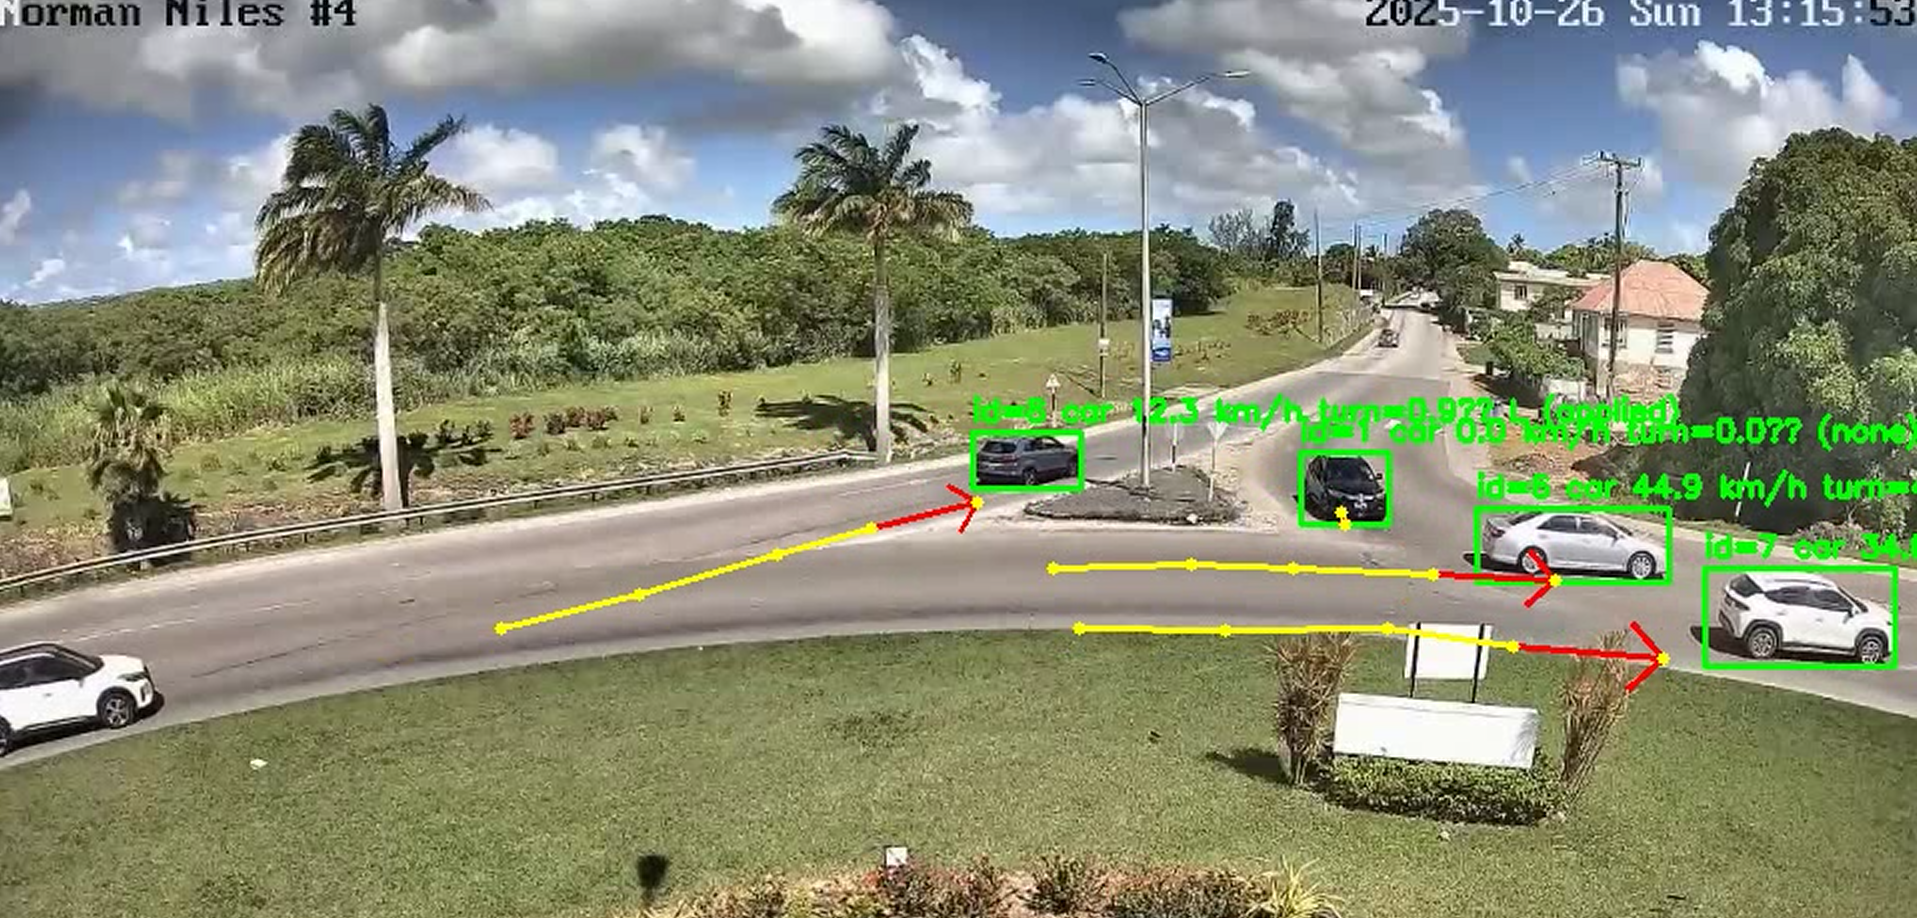
\includegraphics[width=\textwidth]{images/speedcaroverlay.png}
\caption{Real-time speed estimation output. The system maps pixel displacement to real-world coordinates to calculate accurate velocity.}
\label{fig:trajectory}
\end{figure}


\section{System Design \& Architecture}
This section presents the high-level diagrams that serve as the "Blueprint" for the entire EYE-D solution.

\subsection{EYE-D System Design (Deployment Architecture)}
As illustrated in Figure~\ref{fig:system_arch}, the EYE-D system architecture operates as a dedicated Edge-AI deployment map. The operational flow begins with an Industrial Camera capturing real-time RTSP video streams, which are routed to a local Neural Processing Unit (NPU) for low-latency YOLO inference. Following the on-device processing, the extracted metadata (speed, heading, and hazard alerts) are securely transmitted to the EYE-D Web Dashboard.

\begin{figure}[htbp]
  \centering
  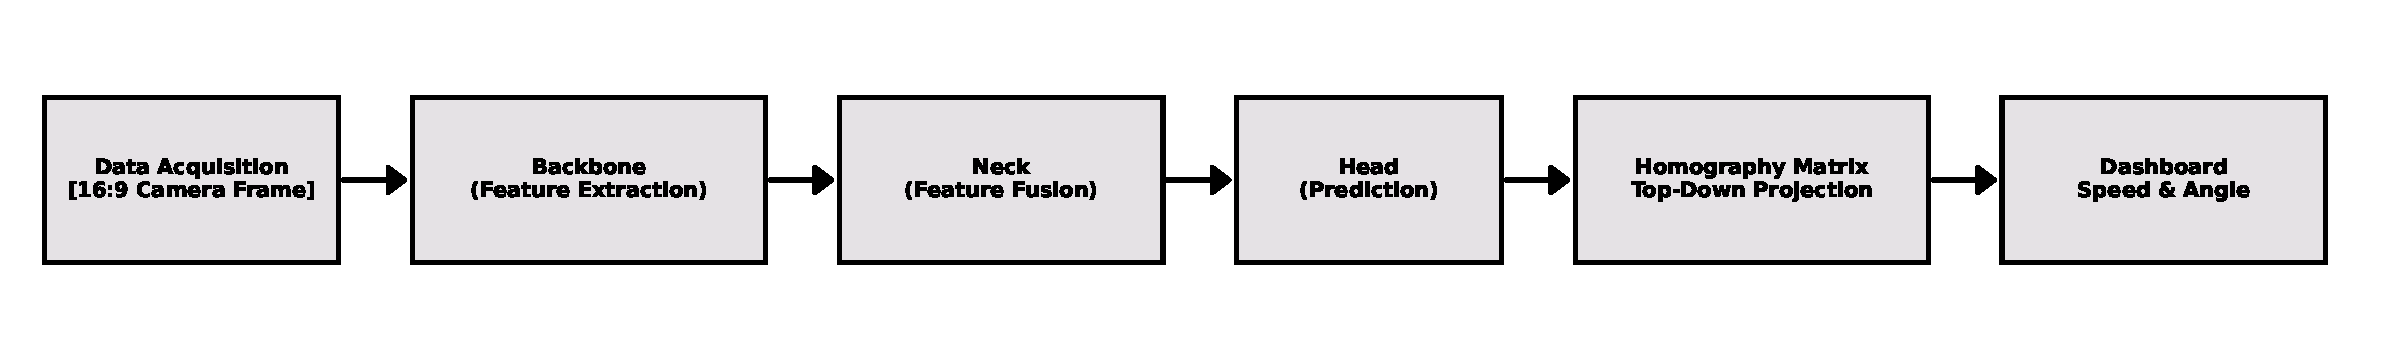
\includegraphics[width=\textwidth]{images/system_architecture.pdf}
\caption{EYE-D System Architecture (Edge-AI Deployment Map).}
\label{fig:system_arch}
\end{figure}

\subsection{Integration \& Multi-Camera Architectures}
To provide a complete engineering blueprint, the system also defines how multiple camera feeds are ingested and processed synchronously.

The UML Integration Architecture specifies the critical interaction between the Video Ingestion module, the NPU Inference Engine, and the Web Dashboard. Specifically, the Video Ingestion module handles the concurrent buffering of multiple RTSP streams, decoding frames directly into NPU-accessible memory space. The NPU Inference Engine then pulls these frames, executing YOLO-based detection and Homography tracking in real time. Finally, the metadata payload-containing timestamps, bounding boxes, object velocities, and alert flags-is serialized and transmitted via WebSockets to the centralized Dashboard, ensuring low-latency situational awareness without overwhelming the network with raw video data.



\begin{figure}[htbp]
  \centering
  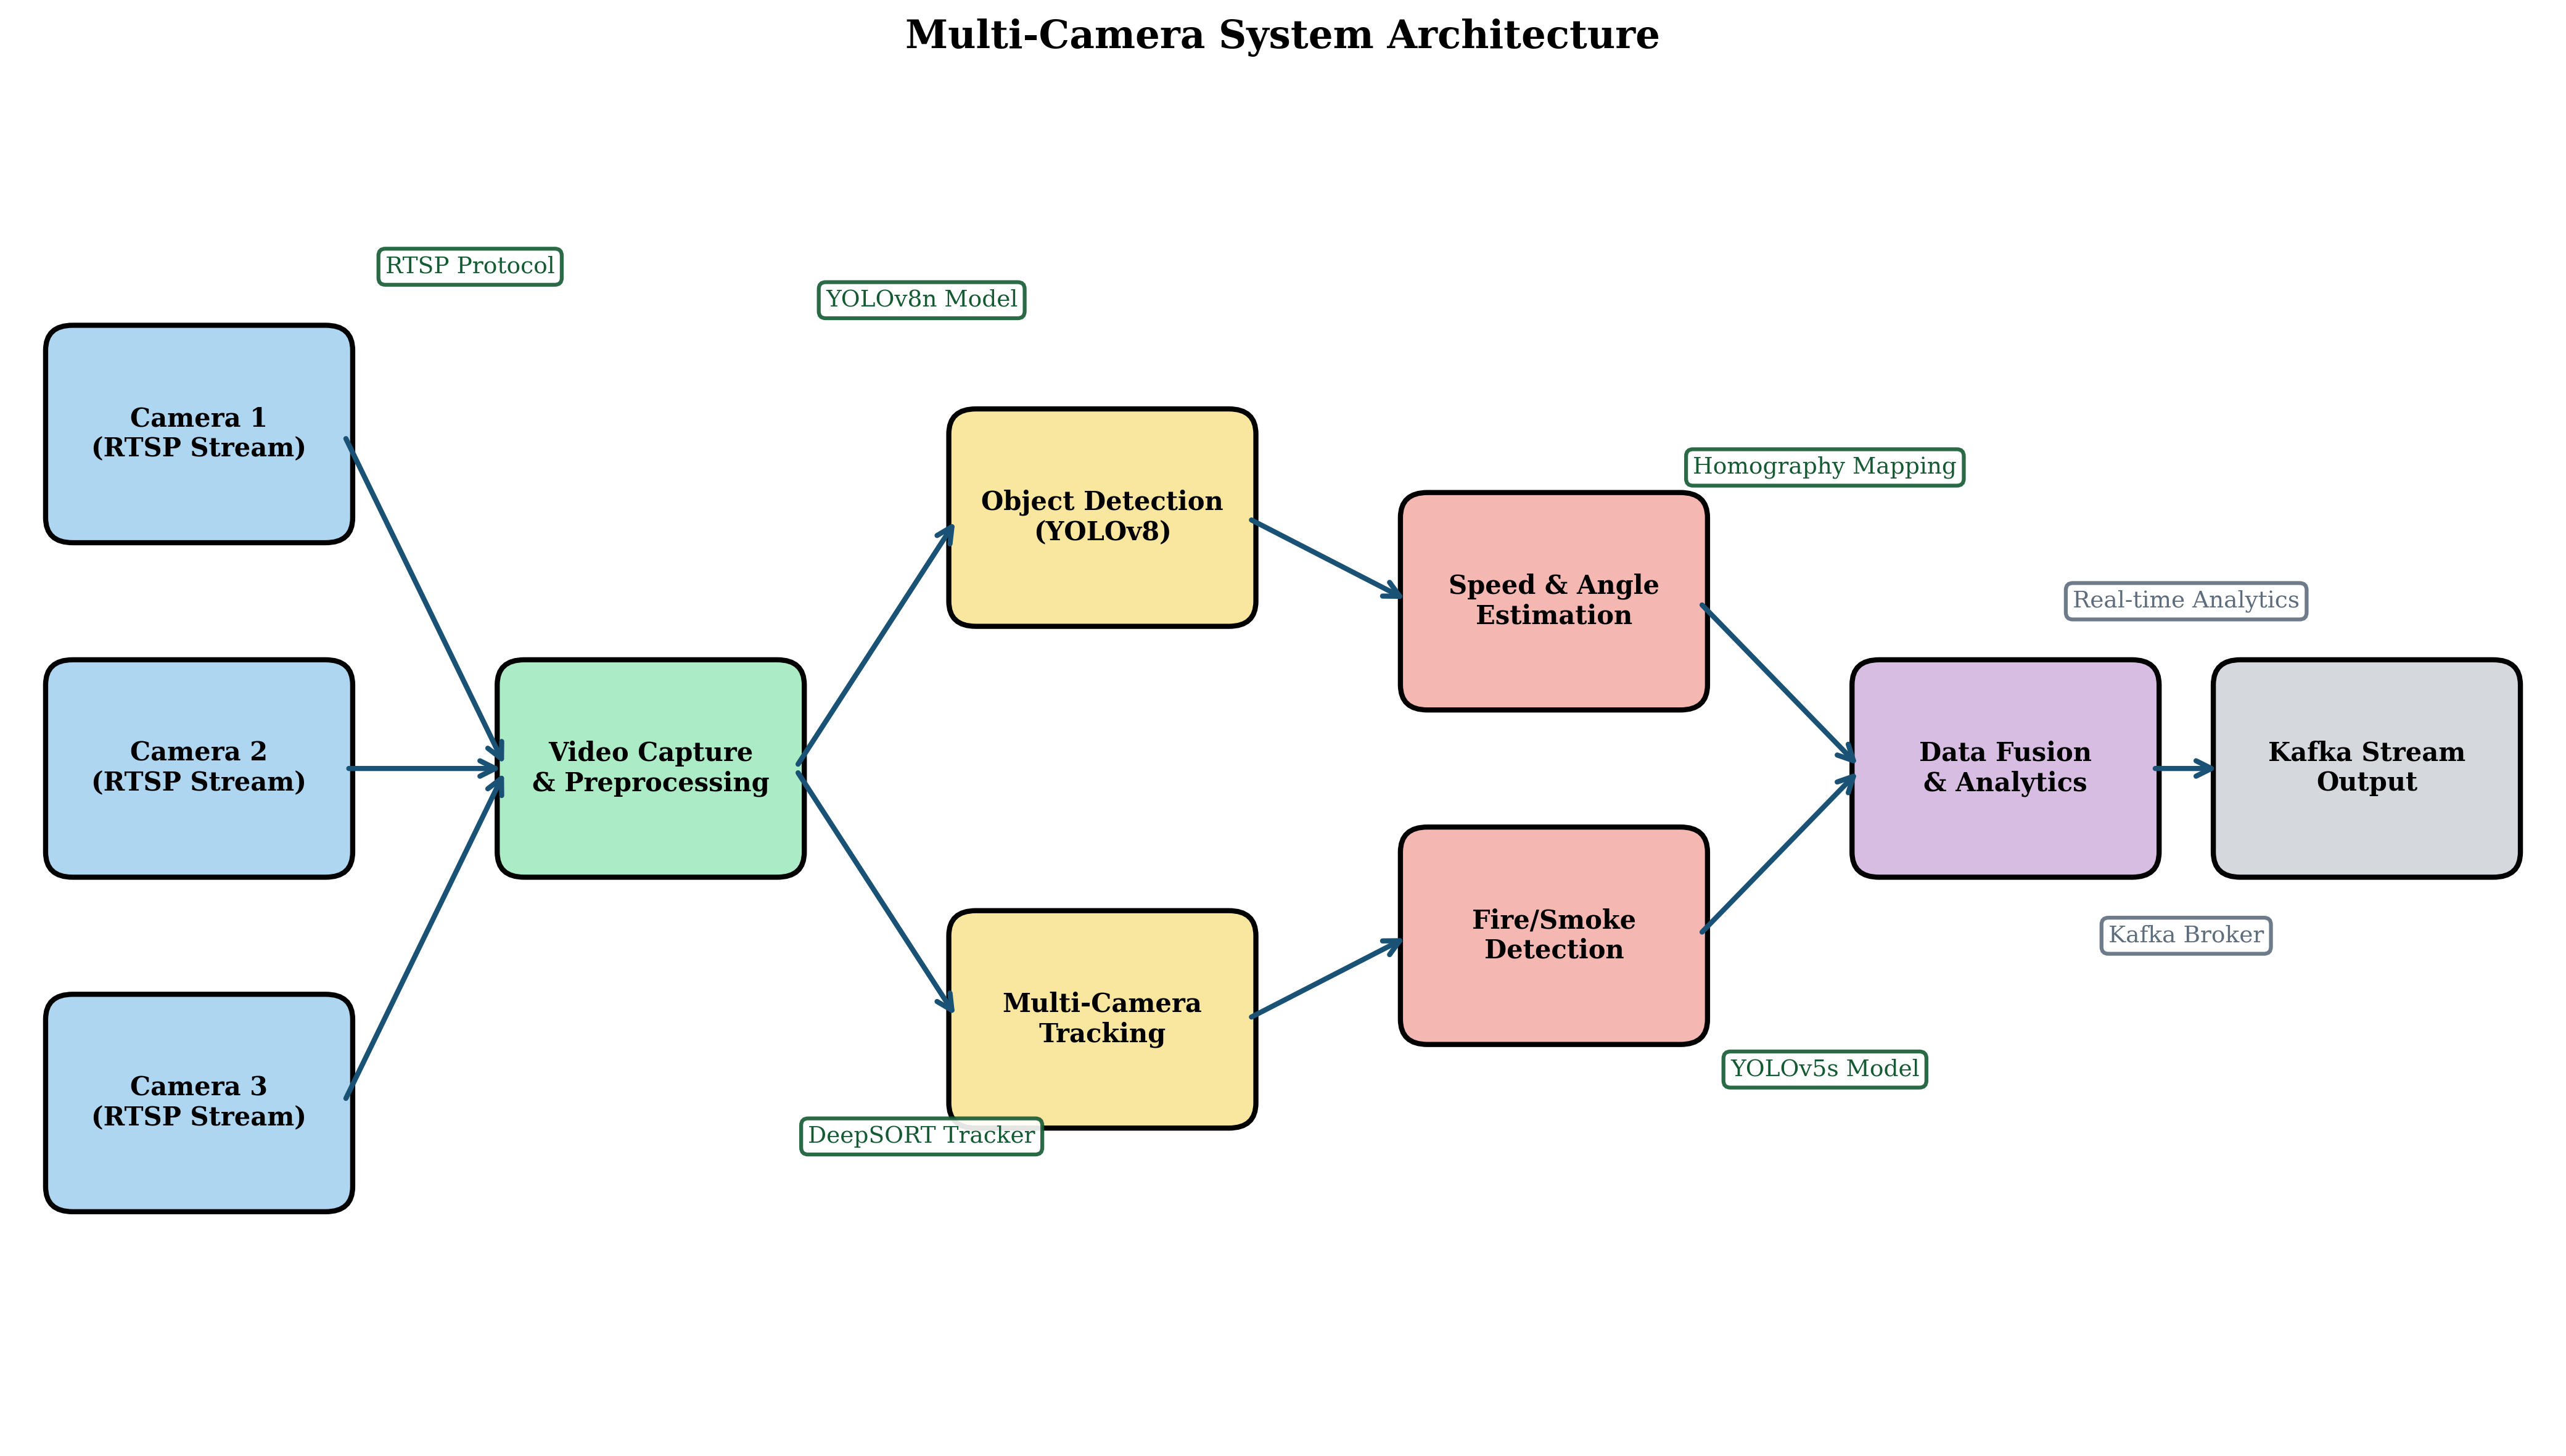
\includegraphics[width=0.8\textwidth]{images/multi_camera_architecture.png}
\caption{Multi-Camera Deployment Architecture for facility-wide monitoring.}
\label{fig:multi_camera_arch}
\end{figure}

\subsection{Workflow Pipeline}
The velocity estimation logic follows a 10-step fullness verification. First, the Homography matrix $\mathbf{H}$ projects 2D image coordinates $(u, v)$ to real-world ground coordinates $(X, Y)$. Then, the instantaneous velocity $v$ is calculated using the formula for Euclidean distance over time between consecutive frames:
\begin{equation}
v = \frac{\sqrt{(X_2-X_1)^2 + (Y_2-Y_1)^2}}{\Delta t}
\end{equation}

\begin{figure}[htbp]
\centering

\includegraphics[width=0.8\textwidth]{images/homography_transform.png}
\caption{Homography-based transformation mapping 2D camera pixels to a top-down ground plane, resolving perspective distortion.}
\label{fig:homography_workflow}
\end{figure}

\begin{figure}[htbp]
\centering
\begin{tikzpicture}[
  node distance=1.5cm and 2cm,
  box/.style={draw, rectangle, rounded corners, align=center, minimum width=2.5cm, minimum height=1cm, fill=blue!10},
  arrow/.style={thick, ->, >=stealth}
]
  \node[box] (cam) {RTSP Camera Feed};
  \node[box, right=of cam] (yolo) {YOLOv5n\\Detection};
  \node[box, right=of yolo] (track) {ByteTrack\\Object Tracking};
  \node[box, below=of track] (homo) {Homography\\Projection};
  \node[box, left=of homo] (speed) {Velocity \& Angle\\Calculation};
  \node[box, left=of speed] (ema) {EMA\\Smoothing};
  
  \draw[arrow] (cam) -- (yolo);
  \draw[arrow] (yolo) -- (track);
  \draw[arrow] (track) -- (homo);
  \draw[arrow] (homo) -- (speed);
  \draw[arrow] (speed) -- (ema);
\end{tikzpicture}
\caption{Speed estimation horizontal workflow pipeline mapping the sequence from YOLO detection to Homography projection and EMA smoothing.}
\label{fig:speed_estimation_workflow}
\end{figure}

\begin{figure}[h]
\centering

\includegraphics[width=\textwidth]{images/workflow_comparison.png}
\caption{Comparison of different speed estimation workflows, highlighting the superiority of Homography for fixed industrial cameras.}
\label{fig:workflow-comparison}
\end{figure}

\section{Chapter Summary}
This chapter detailed the logistical intelligence capabilities of the system. By leveraging mathematical geometric projections (Homography) and temporal smoothing techniques (Kalman Filters and EMA), the EYE-D system successfully transitions from static hazard detection to dynamic behavioral analysis. The presented system architecture diagrams provide a comprehensive blueprint of how these algorithms are orchestrated on the edge to deliver real-time logistical insights while operating strictly within the SRAM and thermal budgets of the NPU hardware.



